\documentclass[../main.tex]{subfiles}
\graphicspath{{\subfix{../images/}}}

\begin{document}

The von neumann architecture specifies a generic structure for CPUs and microprocessors to follow when they are designed. It dictates that the data used to store programs and the data used by the program (tempoary values, variables in memory) should co-exist in the same memory.

To begin, you must understand the main components of a computer.

\subsection{The CPU}
\label{3:sec:cpu}

The CPU or the Central Processing Unit is the brains of your computer. It carries out all the instructions ever passed through your CPU, and is the center of your computer's activity. Modern CPUs have the ability to do many things at once, like playing music while doing word processing\footnote{A very, very, very oversimplified example.}

CPUs look like this:

\begin{figure}[H]
    \centering
    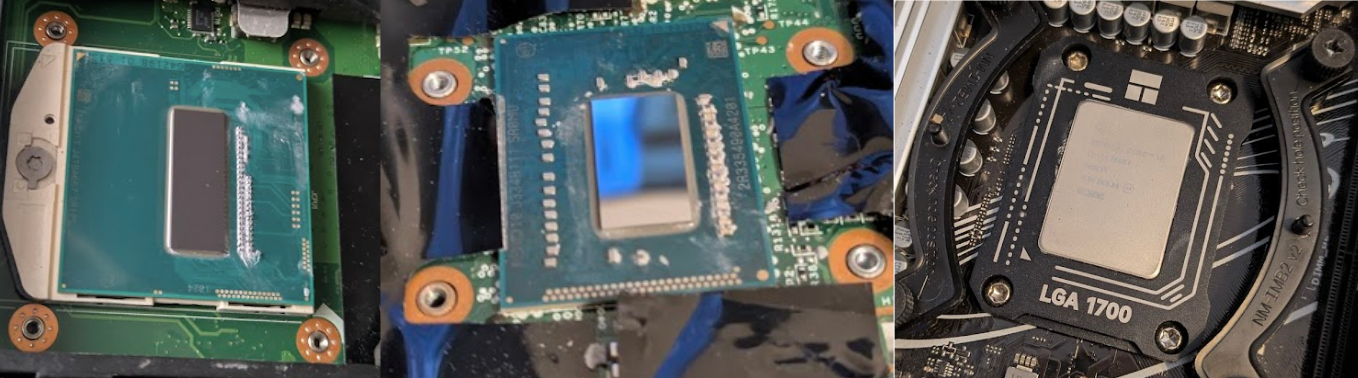
\includegraphics[width=0.85\textwidth]{cpus.png}
    \caption{An Laptop CPU in a socket, an Intel Core i7-4712MQ, a Laptop CPU directly soldered on the motherboard, an Intel Core i7-3520M, and a desktop Intel Core i7-14700KF.}
    \label{fig:cpus}
\end{figure}

\emph{Extra: The shiny part of the CPU is called the die. The die is filled with extremely dense transistors which are all semi-conductive. The die actually does the processing. For those who wonder, no, you cannot see the individual transistors and registers on the CPU; they are so incredibly small and the parts of the CPU are so incredibly small it is impossible to reverse-engineer its architecture; even with microscopes}.

\subsection{Components of a CPU}

\subsection{Buses}

\subsection{The Fetch-Decode-Execute Cycle}

\subsection{The Clock Speed}

\subsection{Increasing CPU speed}

\subsection{Cores}

Cores are like Sub-CPUs in each CPU. Each CPU shown in figure \ref{fig:cpus} has more than 1 core. Each of them can carry out tasks independently of each other; despite how they can communicate together. For those who have already read this whole section, each core can carry out its own fetch-decode-execute cycle.

\begin{figure}[H]
    \centering
    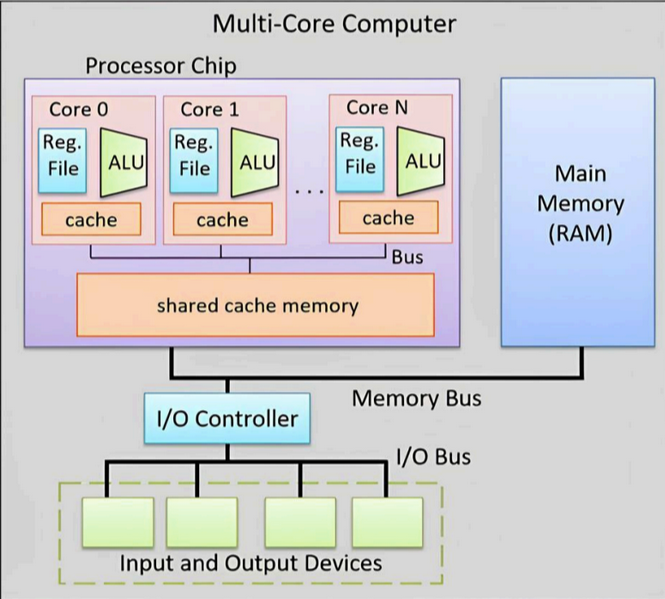
\includegraphics[width=0.7\textwidth]{cores.png}
    \caption{A diagram showing what cores look like in a CPU.}
    \label{fig:cores}
\end{figure}

\end{document}
